\chapter{Planung}
\section{Organisation}
\subsection{Vorgehensweise und Kommunikation}
Zur Planung des Projekts haben wir uns von der agilen Softwareentwicklung und dem Scrum Prinzip inspirieren lassen. Ähnlich wie in Scrum haben wir regelmäßige Treffen mit sogenannten Sprints verbunden. Bei diesen Treffen werden anhand des Projektplans oder Backlogs Aufgaben besprochen und für den Zeitraum bis zum nächsten Treffen entsprechend aufgeteilt. Die Treffen fanden wöchentlich Montags statt. Sie wurden von einem sogenannten 'Srcum-Master' kuratiert, welcher darauf achtet, dass die Besprechungen sachlich bleiben, dass jedes Teammitglied einen Statusbericht abgibt, dass anstehende Probleme und Aufgaben zugewiesen werden und dass die Scrum-Prinzipien eingehalten werden. Die Zeit zwischen den Meetings wird als Sprint bezeichnet und dient dazu, die zugewiesenen Aufgaben zu erledigen. Im reinen Scrum Modell gibt es zusätzlich noch tägliche Meetings, die aber im Rahmen des Semesterprojektes nicht realisierbar waren. Die Kommunikation während der Sprints erfolgte hauptsächlich über den Instant-Messenger WhatsApp. Bei Bedarf gab es auch noch weitere spontan organisierte Treffen um diverse Probleme zu besprechen und sich gegenseitig zu helfen. 

\subsection{Rollenverteilung}
Zu allen Aufgabenbereichen des Projekts wurden Rollen erstellt und jeweils zwei Teammitgliedern zugeordnet. Es gab zu jeder Rolle einen Hauptverantwortlichen und einen Stellvertreter. Die so verteilten Rollen sollten einen Verantwortlichen für jeden Aspekt des Projektes bestimmen, damit bei Problemen oder nachfragen immer eine Ansprechperson gefunden werden kann.

\begin{longtable}[]{|p{.135\textwidth}|p{.17\textwidth}|p{.195\textwidth}|p{.235\textwidth}|p{.22\textwidth}|}
\cline{1-5}
\textbf{Rolle} & \textbf{Beschreibung} &\textbf{Qualifikationen} & \textbf{Verantwortlichkeit} & \textbf{Person} \\ \hline

Projektleiter & 
Operative Planung und Steuerung des Projekts & 
Beherrschen der Projektmanagementinstrumente /
Führen der Gruppe &
Erreichen der Sach- und Terminziele &
1. Kevin Hertfelder
2. Florian Hauger \\ \hline

Dokumenta- tionsbeauftragter &
Dokumentation verwalten /
Zusammentragen /
Protokolle schreiben &
Latexerfahren &
Vollständigkeit und Termineinhaltung der Dokumentationsabgabe &
1. Daniel Petrusic
2. Florian Hauger \\ \hline

Koordinator &
Koordiniert Meetings und sonstige Termine &
&
Termineinhaltung der Meetings &
1. Patrick Kroner
2. Kevin Hertfelder \\ \hline

Architekt / Integrator &
Erstellt Architektur, definiert Schnittstellen & 
Kenntnisse über Software Entwurfsmuster &
Einhaltung der Architektur & 
1. Florian Hauger
2. Kevin Hertfelder \\ \hline

Testverant- wortlicher &
Prüft Testabdeckung & 
Testerfahren &
Korrekte Tests &
1. Daniel Petrusic
2. Patrick Kroner \\ \hline

OpenCV Verantwortlicher &
Implementiert und plant Open CV Funktionalität &
Gute Einarbeitung in OpenCV /
Erfahrung mit Python &
OpenCV Funktionalität &
1. Patrick Kroner
2. Florian Hauger  \\ \hline

Webober- flächen Verantwortlicher &
Implementiert und plant Weboberfläche &
Erfahrung mit Angular und Webtechnologien &
Funktionsumfang und Funktionalität der Weboberfläche &
1. Daniel Petrusic
2. Kevin Hertfelder  \\ \hline

Software- kommunikation und Schnittstellenbeauftragter &
Sorgt für Kommunikation der Softwaremodule &
&
Kommunikation zwischen Kamera und Python /
Kommunikation zwischen Weboberfläche und Python &
1. Kevin Hertfelder
2. Florian Hauger  \\ \hline

System- admin &
Kümmert sich um Ressourcen /
Richtet notwendige Dienste ein &
&
Ressourcen für Entwicklung vorhanden &
1. Florian Hauger
2. Patrick Kroner  \\ \hline

\caption{Rollenverteilung}
\label{tab:rollenverteilung}
\end{longtable}




\subsection{Tools und Technologien}
Die zentrale Bibliothek für das Projekt ist OpenCV. Diese ist Open Source und ermöglicht es, digitale Bildbearbeitung und -analysen einfach und effizient durchzuführen. In unserem Fall war dies notwendig, um die Bewegung in einem Videostream zu erkennen. \newline
OpenCV gibt es für mehrere Sprachen, wobei die am besten unterstützten Sprachen jedoch C++ und Python sind. C++ hätte zwar einen Performance-Vorteil gebracht, andererseits aber etwas kompliziertere Syntax verlangt. Auf Rat des Professors hin, haben wir uns schlussendlich für die Variante mit Python entschieden. \newline
Für die Weboberfläche, haben wir das ebenfalls mit einer Open-Source-Lizenz vertriebene Framework Angular ausgewählt, da dieses moderne Frontend-Entwicklung mit einfacher Datenbindung erlaubt.\newline
Die Sprache der Wahl für die Entwicklung eines Angular-Clienten ist Typescript, welches eine Javascript-Erweiterung ist.\newline
Für die Revisionssicherheit des Projekts wurden drei Git Projekte angelegt.
Die drei Projekte teilten Das Gesamtprojekt in Frontend, Backend und Dokumentation auf. Diese klare Trennung erleichterte paralleles arbeiten am Projekt. Als Hostingprovider für diese Repositories wurde Github gewählt.\newline
Die vewendete Entwicklungsumgebung wurde allen Teammitgliedern frei gestellt und es wurde dann für die Entwicklung am Backend für Python PyCharm von IntelliJ verwendet. Das Typescript Frontend wurde mit Microsoft Visual Studio Code entwickelt.\newline
für die Planung der REST-Schnittstelle haben wir Swagger verwendet.\newline
Für Den Projektplan haben wir Microsoft Projekt verwendet, da wir dieses schon im  Modul Projektmanagement kennen gelernt haben.\newline
Für die Erstellung der Teilpräsentationen wurde Microsoft Powerpoint verwendet.\newline
Schaubilder und Diagramme haben wir mit Microsoft Visio erstellt.\newline
Die Plakate für die Abschlussmesse haben wir mit dem Grafikprogramm Gimp entworfen.\newline

\section{Spezifikation}
\subsection{Anforderungsanalyse}
Die Anforderungen für das Projekt haben wir nach dem Kick-Off Meeting mit dem Professor in einem Kollektiven Brainstorming gesammelt. Da bei diesem Projekt kein klassischer Kunde vorhanden ist, der die grundlegenden Anforderungen vorgibt, waren die Anforderungen recht flexibel und wir haben uns an einigen Referenzprodukten und deren Funktionsumfang orientiert.
\subsection{Anforderungsdetails}
\textbf{Bewegungserkennung}\newline
Ein Videostream soll programmatisch auf Bewegungen überprüft werden. Die Überprüfung soll kleine Änderungen wie durch Wind bewegte Blätter und Kamerarauschen ignorieren und größere Bewegungen erkennen.
\newline
\textbf{Log}\newline
Erkannte Bewegungen sollen in einem Log festgehalten und archiviert werden.
Dabei soll der Zeitpunkt der Aufnahme, die Aufnahme selbst und ein dazugehörendes Thumbnail gespeichert werden. Der Log Wird automatisch erzeugt und kann durch manuelles löschen von Einträgen manipuliert werden.
\newline
\textbf{Aufnahmefunktion}\newline
Wenn eine Bewegung erkannt wurde soll das System in der Lage sein, den Videostream in einer persistenten Datei zu speichern.
Die gespeicherten Aufnahmen müssen jederzeit abrufbar sein.
In der Aufnahme sollen erkannte Bewegungen visuell hervorgehoben werden.
\newline
\textbf{E-Mailbenachrichtigungen}\newline
Bei Einer erkannten Bewegung soll Das System in der Lage sein, automatisiert eine E-Mailbenachrichtigung zu versenden.
\newline
\textbf{lokales Verfahren}\newline
Die aufgezeichneten Daten sollen das lokale Netzwerk nicht verlassen.
Alle Verfahrensschritte benutzen ausschließlich lokal ausgeführte Software.
\newline
\textbf{Videofeed}\newline
Der Videostream soll direkt angezeigt werden können.
\newline
\textbf{Backup}\newline
Es soll die Möglichkeit bestehen, die im Log gesammelten Daten als Archiv zu exportieren.
\newline
\textbf{Einstellungsmöglichkeiten}\newline
In der Weboberfläche sollen einige benutzerspezifische Einstellungen für das Programm getroffen werden können.
Diese umfassen: 
\begin{itemize}
\item Einstellen der Empfindlichkeit der Bewegungserkennung
\item Bildkorrektureigenschaften wie Kontrast und Helligkeit
\item Einstellen der Streamquelle
\item Limit für die maximale Länge einer zusammenhängenden Aufnahme bei konstanter Bewegung
\item Limits für das Backup (maximale Anzahl Dateien / Dateigröße)
\item Festlegen der Empfänger für die E-Mail-Benachrichtigung.
\item Ein-/ausschalten des Logs
\item Ein-/ausschalten der E-Mailbenachrichtigungen
\end{itemize}
\textbf{Weboberfläche}\newline
Es soll eine Weboberfläche als Benutzerschnittelle geschaffen werden die alle Funktionen des Systems einem Anwender zur Verfügung stellt.
Die Funktionen der Weboberfläche sind wie folgt definiert:
\begin{itemize}
\item Der Zugriff soll durch einen Login mit Benutzernamen und Passwort geschützt werden.
\item Der Livefeed der Kamera soll prominent auf der Hauptseite dargestellt werden.
\item Der Log soll mit allen oben definierten Eigenschaften präsentiert werden.
\item Aufnahmen sollen angesehen werden können
\item Alle oben definierten Einstellungen sollen über die Weboberfläche manipuliert werden können.
\item Möglichkeit ein Backup zu erstellen und herunterzuladen.
\end{itemize}
Es gab noch weitere Anforderungen die, wie sich später herausstellte, nicht realisierbar waren. Eine Gesichtserkennung, die wegen der geringen Qualität und Größe der Gesichter in der Aufnahme technisch nicht umsetzbar war.  Zuletzt eine Portierung auf einen Raspberry Pi, die wegen des hohen Leistungsanspruches der Software nicht umsetzbar war. Die Portierung des Produktivsystems erfolgt stattdessen auf einen lokalen Server.
 
\subsection{User Stories}
\begin{itemize}
\item
Als Benutzer möchte ich mich mit einem Benutzernamen und Passwort in die Weboberfläche einloggen, um sicherzustellen, dass nur autorisierte Benutzer Zugriff auf die Weboberfläche haben.
\item
Als Benutzer möchte ich, dass ich Einstellung für die Software über die Weboberfläche ändern kann, um das Softwareverhalten dynamisch zu beeinflussen.
\item
Als Benutzer möchte ich meine E-Mail-Adresse zum Verteiler für Benachrichtigungen hinzufügen und wieder entfernen können, um so einfach wie möglich auf erkannte Bewegungen aufmerksam gemacht zu werden.
\item
Als Benutzer möchte ich Aufnahmen über die Weboberfläche einsehen können, um zu entscheiden, ob die erkannte Bewegung von einem unbefugten Zutritt herrührt.
\item
Als Benutzer möchte ich den Überwachungs-Videostream über eine Weboberfläche einsehen können, um das Blickfeld der Kamera zu sehen.
\item
Als Benutzer möchte ich eine Übersicht über alle erfassten Ereignisse der Kamera mit Zeitstempel einsehen, um nach einem Event in einem gewissen Zeitraum zu suchen.
\item
Als Benutzer möchte ich, dass meine Daten nicht auf den Servern von Drittanbietern gespeichert werden, um meine Privatsphäre zu schützen.
\item
Als Benutzer möchte ich, die gesammelten Aufnahmedaten exportieren, um sie anderweitig zu verwenden.
\end{itemize}

\subsection{Projektplanung und Meilensteine}
Die Termine der Meilensteine wurden an den Zweiwöchentlichen Meetings mit den Betreuern ausgerichtet. Einzige Ausnahme war die Implementierungsphase, welche für die Basisimplementierung vier Wochen beansprucht hat. Somit ergeben sich Meilensteine für die, unter anderem im klassischen Wasserfallmodell, vorgegebenen Phasen Spezifikation, Entwurf, Implementierung sowie Test. Ein letzter, zusätzlicher Meilenstein für die abschließende Präsentation und Abgabe. Die Implementierungsphase war jedoch in  drei feingranulare Meilensteine aufgeteilt. Es wurden zwei Meilensteine für die Basisfunktionalität von Front- beziehungsweise Backend und die Featureimplementierung aufgestellt. Arbeit an den Meilensteinen von Front- und Backend konnten parallel bearbeitet werden. Zur Gewichtung der Projektphasen war uns bewusst, dass im Idealfall mehr Zeit für die Spezifikation und den Entwurf nötig gewesen wäre, jedoch war in der begrenzten Zeit, welche dem Semesterprojekt zur Verfügung stand, die Implementierung im Vordergrund. Sie nimmt in unserem Fall ungefähr die Hälfte der Gesamtzeit in Anspruch.
\newpage
\begin{figure}[h]
	\centering
	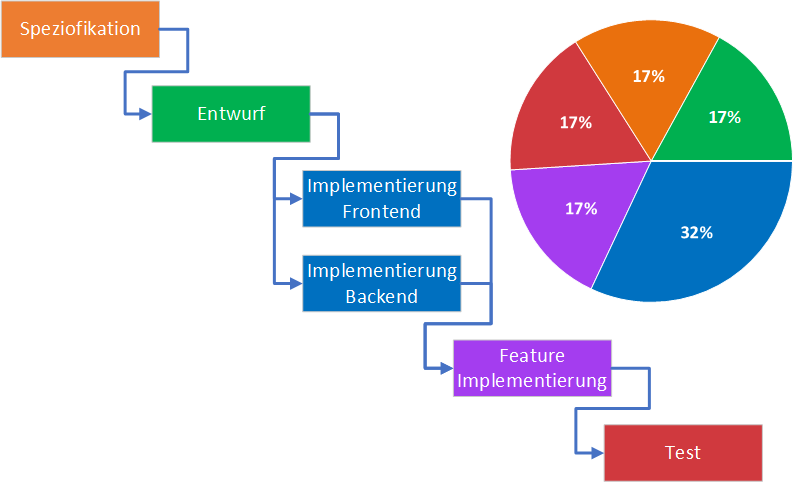
\includegraphics[width=\textwidth]{content/pictures/Phasen_Diagramm.png}
	\caption{Meilensteindiagramm}
	\label{img:milestone}
\end{figure}

Die Meilensteine konnten im Projektverlauf ausnahmslos eingehalten werden und es gab daher keine Verschiebungen.

\section{Entwurf}
\subsection{Systemarchitektur}
Bei dem ersten Treffen mit dem 'Kunden' wurde von uns eine Software zur Überwachung eines Raumes mithilfe einer herkömmlichen IP-Kamera gewünscht.
Da hierfür auch eine Möglichkeit zur Interaktion mit dem System gegeben sein sollte, entschieden wir uns für eine Webseite, mit welcher der Videofeed sichtbar gemacht wird und Einstellungen vorgenommen werden können. Da die Software im Gegensatz zu anderen kommerziellen Produkten im lokalen Netz bleiben sollte,
spielte die Sicherheit keine große Rolle.\\
Die Architektur sollte die Aufteilung der Schichten wie Logik, Datenhaltung sowie die Präsentation durch den Webserver darstellen.
Hierfür wurde zuerst Abbildung \ref{img:architecture-sketch} erstellt.\\\\
\begin{figure}[h]
	\centering
	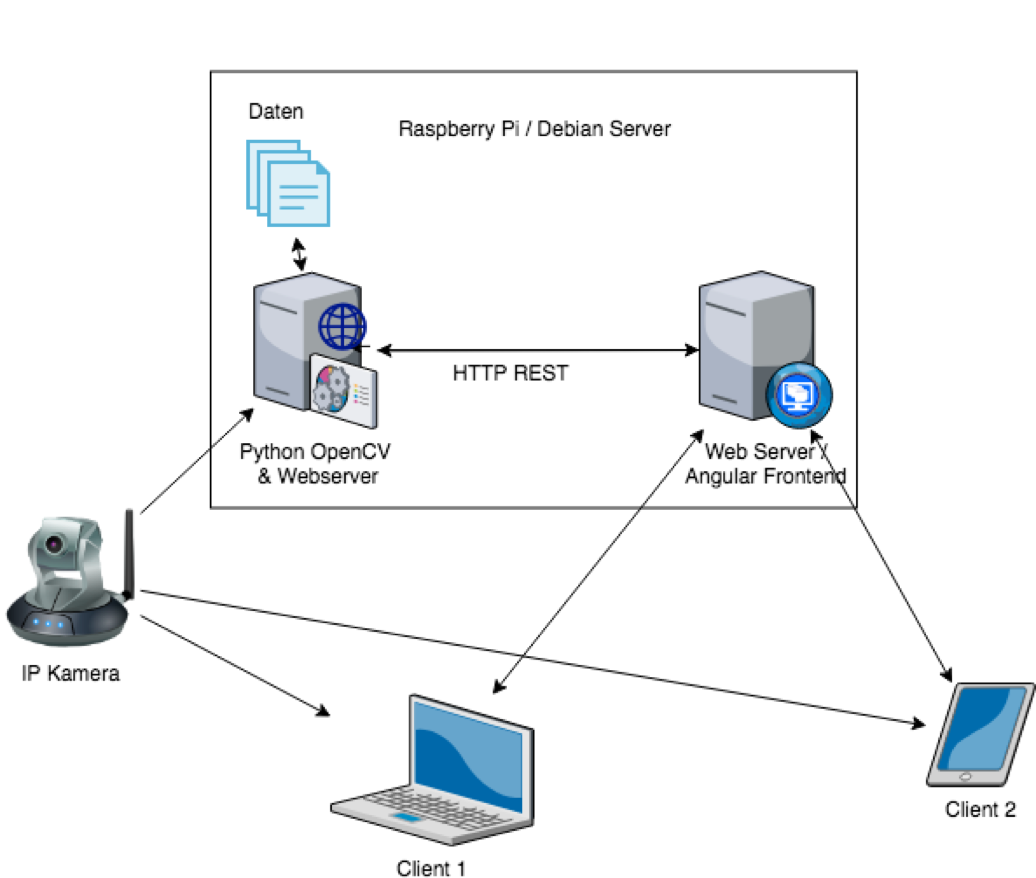
\includegraphics[height=10cm]{content/pictures/architecture-sketch.png}
	\caption{Erste Planung der Architektur}
	\label{img:architecture-sketch}
\end{figure}
Da der Architekt im Gebiet der Webtechnologien kaum Erfahrung hatte, entschieden die verantwortlichen Entwickler sich selbst für Angular und sprachen sich bei
der Entwicklung ab. Lediglich REST wurde für die Kommunikation zwischen Frontend und Backend definiert. 
Um die Aufteilung der Klassen und Kommunikation innerhalb des Backends darzustellen wurde ein vereinfachtes Klassendiagramm erstellt (Abbildung \ref{img:backend-classdiagramm}).\\
Die Klasse für die Bildverarbeitung sowie die Klasse für die REST-Schnittstellen besitzen eine eigene run-Methode und laufen in einem gesonderten Thread. Diese Methoden werden innerhalb der Main-Klasse ausgeführt. Die Daten sind innerhalb der ImageProcessing-Klasse und des Webservers verfügbar. Es gibt außerdem jeweils eine weitere Klasse für das Versenden der Email-Benachrichtigung sowie für die permanente Ablage der Daten.\\\\
\begin{figure}[]
	\centering
	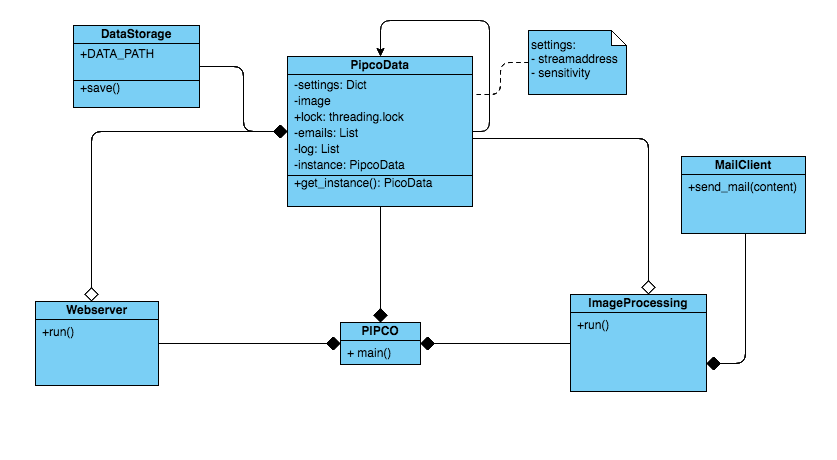
\includegraphics[width=\textwidth]{content/pictures/classdiagramm.png}
	\caption{Klassendiagramm: Aufbau des Backends}
	\label{img:backend-classdiagramm}
\end{figure}

Während der Entwicklung stellte sich heraus, dass der Aufwand für die Implementierung der bidirektionalen Kommunikation zwischen Frontend und Backend zu hoch ist, weshalb wir uns dazu entschieden die Daten direkt vom Backend zu holen und die Logs mithilfe von Polling aktuell zu halten.
Eine weitere Änderung war die Kamera, welche lediglich vom Backend angefragt wird. Der Client sollte sich ausschließlich die Bilder mit eingezeichneten Bewegungen holen.
Hierdurch änderte sich die Architektur wie in Abbildung \ref{img:architecture-change} zu sehen.\\

Um den Ablauf der Implementierten Version besser nachvollziehen zu können wurde ein Sequenzdiagramm erstellt (Abbildung \ref{img:sequencediagram}).

\begin{figure}[]
	\centering
	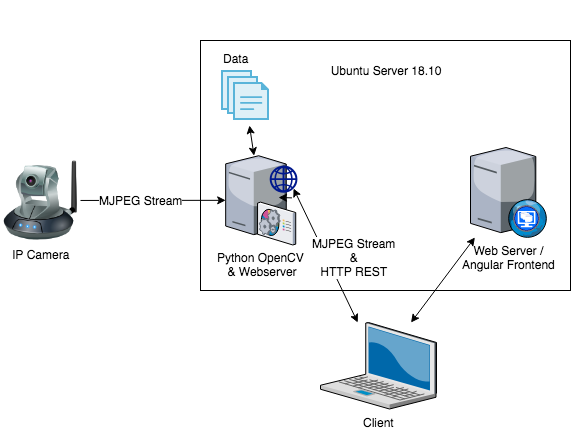
\includegraphics[width=\textwidth]{content/pictures/architecture-change.png}
	\caption{Architektur: Direkter Zugriff auf das Backend}
	\label{img:architecture-change}
\end{figure}

\begin{figure}[]
	\centering
	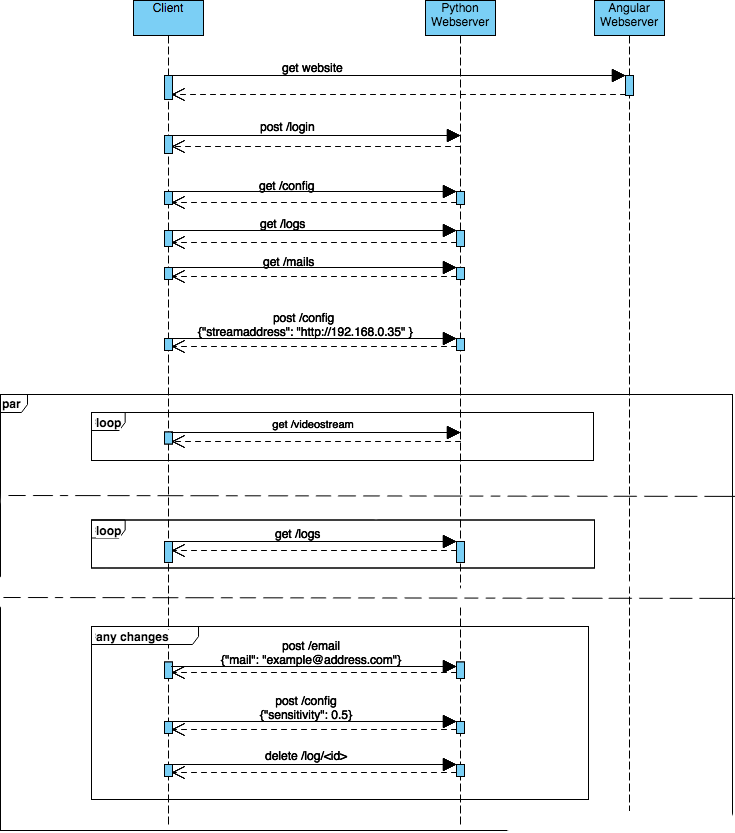
\includegraphics[width=\textwidth]{content/pictures/sequencediagram.png}
	\caption{Ablauf Login und Änderungen}
	\label{img:sequencediagram}
\end{figure}

\subsection{Rest Schnittstelle}
Für die Unabhängige Entwicklung der Kommunikation von Frontend und Backend wurde eine Liste mit den notwendigen REST-Nachrichten erstellt (Tabelle \ref{table:kommunikation}).\\\\
\begin{table}[]
	\centering
	\caption{Kommunikation Backend und Frontend}
	\label{table:kommunikation}
	\resizebox{\textwidth}{!}{\begin{tabular}{llll}
			\textbf{Type} & \textbf{address}                                                             & \textbf{keys}                                                                                                                                                                                                                                          & \textbf{returns}           \\
			POST          & /login                                                                       & user, password                                                                                                                                                                                                                                         & OK / Error 403             \\
			GET           & /videostream                                                                 &                                                                                                                                                                                                                                                        & mjpeg stream               \\
			GET           & /logs/\textless{}page\_no\textgreater{}/\textless{}batch\_size\textgreater{} &                                                                                                                                                                                                                                                        & list with logs             \\
			DELETE        & /log/\textless{}log\_id\textgreater{}                                        &                                                                                                                                                                                                                                                        & id / Error 403             \\
			POST          & /mail                                                                        &                                                                                                                                                                                                                                                        & id / Error 403             \\
			GET           & /mails                                                                       &                                                                                                                                                                                                                                                        & list of mail addresses     \\
			DELETE        & /mail/\textless{}mail\_id\textgreater{}                                      &                                                                                                                                                                                                                                                        & id / Error 403             \\
			PUT           & /mail/\textless{}mail\_id\textgreater{}                                      &                                                                                                                                                                                                                                                        & notify status / Error 403  \\
			POST          & /config                                                                      & \multirow{4}{*}{\begin{tabular}[c]{@{}l@{}}sensitivity(float), streamaddress,brightness (float),\\ contrast (float), log\_enabled(bool),\\ global\_notify(bool), cliplength (int in seconds),\\ max\_logs (int),max\_storage (int in MB)\end{tabular}} & changed values / Error 403 \\
			&                                                                              &                                                                                                                                                                                                                                                        &                            \\
			&                                                                              &                                                                                                                                                                                                                                                        &                            \\
			&                                                                              &                                                                                                                                                                                                                                                        &                            \\
			GET           & config                                                                       &                                                                                                                                                                                                                                                        & config                     \\
			GET           & /recording/\textless{}filename\textgreater{}                                 &                                                                                                                                                                                                                                                        & videofile                  \\
			GET           & /backup                                                                      &                                                                                                                                                                                                                                                        & backup.zip                 \\
			&                                                                              &                                                                                                                                                                                                                                                        &                           
		\end{tabular}}
	\end{table}